\documentclass[12pt]{article}
\usepackage{color}
\usepackage{multicol,ifthen,booktabs,amsmath,amsfonts,bm,mathrsfs,amssymb}
\usepackage{times,mathptmx}
\usepackage{braket}
\usepackage{enumerate}
\usepackage{geometry}
\usepackage{graphicx}% Include figure files
\usepackage{listings}
\usepackage[latin1]{inputenc}
\usepackage{tikz}
\usepackage{tikz-feynman}
\usetikzlibrary{trees}
\usetikzlibrary{decorations.pathmorphing}
\usetikzlibrary{decorations.markings}
\usepackage{verbatim}
\renewcommand\baselinestretch{1.5}\protect
\abovedisplayshortskip 3 pt
\belowdisplayshortskip 3 pt
\geometry{left=2cm,right=2cm,top=3cm,bottom=3cm}
\graphicspath{{./figures/}{./}}

% Define styles for the different kind of edges in a Feynman diagram
\tikzset{
    fermion/.style={draw=black, postaction={decorate},
        decoration={markings,mark=at position .55 with {\arrow[draw=black]{>}}}},
    fermionbar/.style={draw=black, postaction={decorate},
        decoration={markings,mark=at position .55 with {\arrow[draw=black]{<}}}},
    fermionnoarrow/.style={draw=black},
    gluon/.style={decorate, draw=orange,
        decoration={coil,amplitude=3pt, segment length=4pt}},
    scalar/.style={dashed,draw=red},
    scalarpi/.style={dashed,draw=blue},
}

\begin{document}

\section{Flow equation}
\begin{eqnarray}
\begin{split}
\partial_t \Gamma_k  \sim & \partial_t \{ \bar q (Z_{q,k} i \gamma_{\mu} q_{\mu}+ m_f) q \} \\
= &- \tilde{\partial_t}
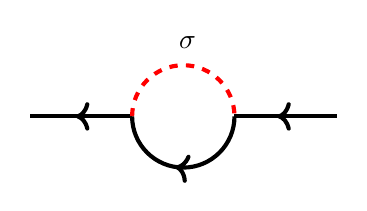
\begin{tikzpicture}[line width=1.5 pt, scale=1.3]
	\draw[fermion] (0:1)--(0,0);
	\draw[scalar] (1,0) arc (180:0:.5);
          \draw[fermion] (2,0) arc (0:-180:.5);
	\draw[fermionbar] (2,0) --(3,0);
          \node  at (25:1.7) {$\sigma$};
\end{tikzpicture}\\
&- \tilde{\partial_t}
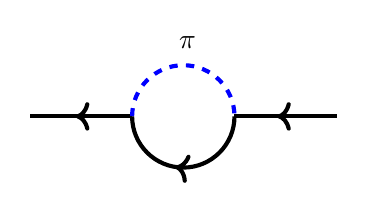
\begin{tikzpicture}[line width=1.5 pt, scale=1.3]
	\draw[fermion] (0:1)--(0,0);
	\draw[scalarpi] (1,0) arc (180:0:.5);
	\draw[fermion] (2,0) arc (0:-180:.5);
	\draw[fermionbar] (2,0) --(3,0);
          \node  at (25:1.7) {$\pi$};
\end{tikzpicture}\\
&- \tilde{\partial_t}
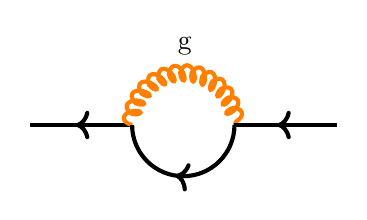
\begin{tikzpicture}[line width=1.5 pt, scale=1.3]
	\draw[fermion] (0:1)--(0,0);
	\draw[gluon] (1,0) arc (180:0:.5);
	\draw[fermion] (2,0) arc (0:-180:.5);
          \node  at (27:1.7) {g};
	\draw[fermionbar] (2,0) --(3,0);
\end{tikzpicture}
\end{split}
\end{eqnarray}
\begin{eqnarray}
\begin{split}
\eta_q^\sigma=&
-\frac{1}{Z_{q,k}} \frac{1}{p^2} \tilde{\partial_t} \Bigg ( \frac{1}{4} tr \Bigg (i \vec{p}\cdot \vec{\gamma}
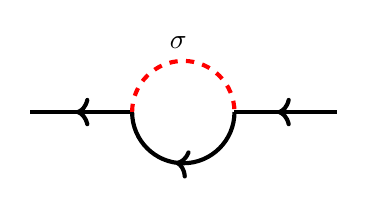
\begin{tikzpicture}[line width=1.5 pt, scale=1.3]
	\draw[fermion] (0:1)--(0,0);
	\draw[scalar] (1,0) arc (180:0:.5);
          \draw[fermion] (2,0) arc (0:-180:.5);
	\draw[fermionbar] (2,0) --(3,0);
          \node  at (25:1.6) {$\sigma$};
\end{tikzpicture}
\Bigg )\Bigg |_p
%-\frac{1}{4} tr \Bigg (i \vec{p}\cdot \vec{\gamma}
%\begin{tikzpicture}[line width=1.5 pt, scale=1.3]
%	\draw[fermion] (0:1)--(0,0);
%	\draw[scalar] (1,0) arc (180:0:.5);
 %         \draw[fermion] (2,0) arc (0:-180:.5);
%	\draw[fermionbar] (2,0) --(3,0);
%          \node  at (25:1.6) {$\sigma$};
%\end{tikzpicture}
%\Bigg )\Bigg |_{p=0} 
\Bigg )\\
=& - \frac{1}{Z_{q,k}} \frac{1}{p^2} \tilde{\partial_t}\sum \!\!\!\!\!\!\!\!\!\int \Bigg ( \frac{1}{Z_{\phi,k} Z_{q,k}}\frac{h^2_k}{4} (\vec{p} \cdot \vec{q}_F) \bar G^q_k (q) \bar G^{\sigma}_k(q-p) \Bigg )\\
=&- \frac{1}{Z_{\phi,k} Z_{q,k}^2} \frac{1}{p^2}\frac{h^2_k}{4} \sum \!\!\!\!\!\!\!\!\!\int  \bigg ( (\tilde{\partial_t} \vec{q}_F)\cdot  \vec{p} \bar G^q_k (q) \bar G^{\sigma}_k(q-p) +(\vec{q}_F \cdot \vec {p})\tilde{\partial_t}  \bar G^q_k (q) \bar G^{\sigma}_k(q-p)\\
&+(\overrightarrow{q-p})_F \cdot \vec{p} \bar G^q_k (q-p) \tilde{\partial_t}  \bar G^{\sigma}_k(q) \bigg )
\end{split}
\end{eqnarray}
\begin{eqnarray}
(\tilde{\partial_t} q_F) \cdot \vec{p}= \vec{q} (\tilde{\partial_t} r_F ) \cdot \vec{p}=\vec{q}  \cdot \vec{p} \frac{1}{Z_{q,k}} \partial_t(Z_{q,k} r_F)=[(1-\eta_q)x^{-\frac{1}{2}} + \eta_q] \theta(1-x) \vec{q}  \cdot \vec{p}
\end{eqnarray}
\begin{eqnarray}
\tilde{\partial_t}  \bar G^q_k (q) = -2k^2 (\bar G^q_k(q))^2 [(1-\eta_q)+\eta_q x^{\frac{1}{2}}]\theta(1-x)
\end{eqnarray}
\begin{eqnarray}
\tilde{\partial_t}  \bar G^{\sigma}_k (q) = -k^2 (\bar G^{\sigma}_k(q))^2 [(2-\eta_\phi)+\eta_\phi x]\theta(1-x)
\end{eqnarray}
\begin{eqnarray}
\begin{split}
&T \sum_n\int \frac{d^3q}{(2 \pi)^3} (\tilde{\partial_t} \vec{q}_F)\cdot  \vec{p} \bar G^q_k (q) \bar G^{\sigma}_k(q-p) \\
=&T \sum_n \int \frac{d^3q}{(2 \pi)^3}[(1-\eta_q)x^{-\frac{1}{2}} + \eta_q] \theta(1-x) (\vec{q}  \cdot \vec{p}) \frac{1}{k^4} \tilde G^q_k(q) \tilde G^{\sigma}_k(q-p)\\
=& \int \frac{d^3q}{(2 \pi)^3}[(1-\eta_q)x^{-\frac{1}{2}} + \eta_q] \theta(1-x) (\vec{q}  \cdot \vec{p}) \frac{1}{k^3} \frac{T}{k} \sum_n\tilde G^q_k(q) \tilde G^{\sigma}_k(q-p)
\end{split}
\end{eqnarray}
here we note that
\begin{eqnarray}
\begin{split}
&\frac{T}{k} \sum_n \tilde G^q_k(q) \tilde G^{\phi}_k(q-p) \\
&=\mathcal{F}1\mathcal{B}1(m_q;m_{\phi,q-p})
\end{split}
\end{eqnarray}
then
\begin{eqnarray}
\begin{split}
above=& \int \frac{d^3q}{(2 \pi)^3}[(1-\eta_q)x^{-\frac{1}{2}} + \eta_q] \theta(1-x) (q p \cos \theta) \frac{1}{k^3} \mathcal{F}1\mathcal{B}1(m_q;m_{\phi,q-p})\\
&=\frac{p}{(2 \pi)^2}\int _0^{\infty}q^2 dq \int_{-1}^{1} d \cos \theta \frac{1}{k^3} [(1-\eta_q)x^{-\frac{1}{2}} + \eta_q] \theta(1-x) q \cos \theta \mathcal{F}1\mathcal{B}1(m_q;m_{\phi,q-p})\\
&=\frac{p}{(2 \pi)^2}\int _0^{\infty}q^3 dq  \frac{1}{k^3} [(1-\eta_q)x^{-\frac{1}{2}} + \eta_q] \theta(1-x)  \int_{-1}^{1} d \cos \theta \cos \theta \mathcal{F}1\mathcal{B}1(m_q;m_{\phi,q-p})\\
&=\frac{k p}{2 (2 \pi)^2}\int _0^1 x dx  [(1-\eta_q)x^{-\frac{1}{2}} + \eta_q] \int_{-1}^{1} d \cos \theta \cos \theta \mathcal{F}1\mathcal{B}1(m_q;m_{\phi,q-p})\\
&=\frac{k p}{2 (2 \pi)^2}\int _0^1 dx  [(1-\eta_q)x^{\frac{1}{2}} + \eta_q x] \int_{-1}^{1} d \cos \theta \cos \theta \mathcal{F}1\mathcal{B}1(m_q;m_{\phi,q-p})
\end{split}
\end{eqnarray}







%%%%%%%%%%%%%%%%%%%%%%%%%%%%%%%%%%%

\end{document}
